%###############################################################################
%# WbXbc - Manual - Overview                                                   #
%###############################################################################
%#    Copyright 2018 Dirk Heisswolf                                            #
%#    This file is part of the WbXbc project.                                  #
%#                                                                             #
%#    WbXbc is free software: you can redistribute it and/or modify            #
%#    it under the terms of the GNU General Public License as published by     #
%#    the Free Software Foundation, either version 3 of the License, or        #
%#    (at your option) any later version.                                      #
%#                                                                             #
%#    WbXbc is distributed in the hope that it will be useful,                 #
%#    but WITHOUT ANY WARRANTY; without even the implied warranty of           #
%#    MERCHANTABILITY or FITNESS FOR A PARTICULAR PURPOSE.  See the            #
%#    GNU General Public License for more details.                             #
%#                                                                             #
%#    You should have received a copy of the GNU General Public License        #
%#    along with WbXbc.  If not, see <http:%www.gnu.org/licenses/>.            #
%###############################################################################
%# Version History:                                                            #
%#   September 10, 2018                                                        #
%#      - Initial release                                                      #
%###############################################################################

\section{Overview}
\label{overview}

WbXbc stands for ``\textbf{W}ish\textbf{b}one \textbf{cross}\textbf{b}ar \textbf{c}omponents''.
It is a collection of soft IP blocks for building customized crossbar switches.
As all WbXbc blocks interconnect via a common interface (pipelined Wishbone protocol~\cite{wishbone}),
they can be easily arranged to fulfil application specific performance or size requirements.
An example of different ways a set of Wishbone initiators may be connected to a set of Wishbone targets
shown in \figref{overview:diag}. The four implementations differ in the number of concurrent bus accesses
they support and in the amount of logic gates they require. The WbXbc components in this example are
described in \secref{comp}.

\begin{figure}[H]
  %\begin{center}
  \makebox[\textwidth][c]{
    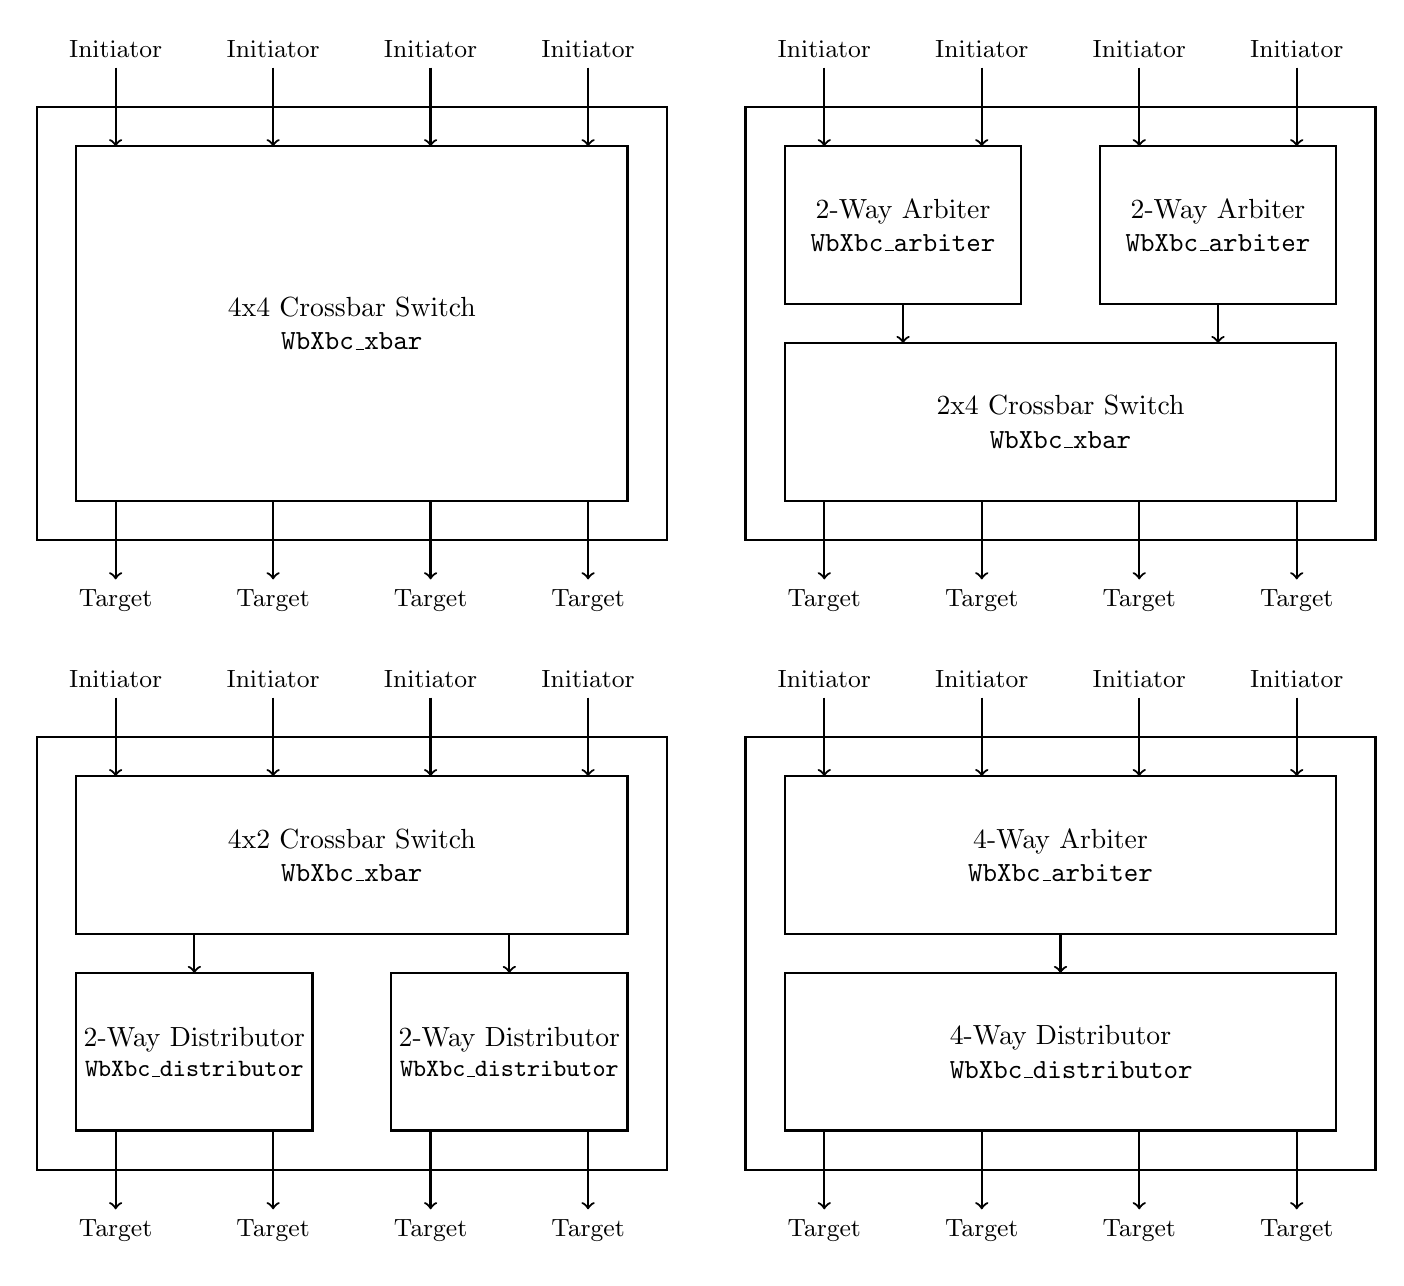
\begin{tikzpicture}

      %\draw [thin, fill=white] (0,0) rectangle (17,15.5);
      \draw[transparent] (0,0) rectangle (17,15.5);

      
      %Top level interfaces
      \newsavebox{\topif}
      \savebox{\topif}{
        \draw [thick, fill=white] (0,1) rectangle (8,6.5);
        \foreach \xpos in {1, 3, 5, 7} {
          \node [above] at (\xpos,7)  {\small{Initiator}};
          \node [below] at (\xpos,0.5){\small{Target}};
          \draw [thick, ->] (\xpos,7) -- (\xpos,6);
          \draw [thick, ->] (\xpos,1.5) -- (\xpos,0.5);
        }
      };
      %4x4 crossbar
      \node at (0,8) {\usebox{\topif}};
      %Xbar 
      \draw [thick, fill=white] (.5,9.5) rectangle (7.5,14);
      \node at (4,11.75)
            {\begin{minipage}[c]{10em}
                \begin{center}
                  \hyphenchar\font=-1
                  4x4 Crossbar Switch \\ 
                  \texttt{WbXbc\_xbar}
                \end{center}
            \end{minipage}};       
      %2x4 crossbar
      \node at (9,8) {\usebox{\topif}};
      %Arbiters
      \draw [thick, fill=white] (9.5,12) rectangle (12.5,14);
      \draw [thick, fill=white] (13.5,12) rectangle (16.5,14);
      \draw [thick, ->] (11,12) -- (11,11.5);
      \draw [thick, ->] (15,12) -- (15,11.5);
      \node at (11,13)
            {\begin{minipage}[c]{8em}
                \begin{center}
                  \hyphenchar\font=-1
                  2-Way Arbiter \\ 
                  \texttt{WbXbc\_arbiter}
                \end{center}
            \end{minipage}};       
      \node at (15,13)
            {\begin{minipage}[c]{8em}
                \begin{center}
                  \hyphenchar\font=-1
                  2-Way Arbiter \\ 
                  \texttt{WbXbc\_arbiter}
                \end{center}
            \end{minipage}};       
      %Xbar 
      \draw [thick, fill=white] (9.5,9.5) rectangle (16.5,11.5);
      \node at (13,10.5)
            {\begin{minipage}[c]{10em}
                \begin{center}
                  \hyphenchar\font=-1
                  2x4 Crossbar Switch \\ 
                  \texttt{WbXbc\_xbar}
                \end{center}
            \end{minipage}};       
      %4x2 crossbar
      \node at (0,0) {\usebox{\topif}};
      %Xbar 
      \draw [thick, fill=white] (0.5,4) rectangle (7.5,6);
      \draw [thick, ->] (2,4) -- (2,3.5);
      \draw [thick, ->] (6,4) -- (6,3.5);
      \node at (4,5)
            {\begin{minipage}[c]{10em}
                \begin{center}
                  \hyphenchar\font=-1
                  4x2 Crossbar Switch \\ 
                  \texttt{WbXbc\_xbar}
                \end{center}
            \end{minipage}};                   
      %Distributors
      \draw [thick, fill=white] (0.5,1.5) rectangle (3.5,3.5);
      \draw [thick, fill=white] (4.5,1.5) rectangle (7.5,3.5);
      \node at (2,2.5)
            {\begin{minipage}[c]{8em}
                \begin{center}
                  \hyphenchar\font=-1
                  2-Way Distributor \\ 
                  \small{\texttt{WbXbc\_distributor}}
                \end{center}
            \end{minipage}};       
      \node at (6,2.5)
            {\begin{minipage}[c]{8em}
                \begin{center}
                  \hyphenchar\font=-1
                  2-Way Distributor \\ 
                  \small{\texttt{WbXbc\_distributor}}
                \end{center}
            \end{minipage}};       
      %no crossbar
      \node at (9,0) {\usebox{\topif}};
      %Arbiter
      \draw [thick, fill=white] (9.5,4) rectangle (16.5,6);
      \draw [thick, ->] (13,4) -- (13,3.5);
      \node at (13,5)
            {\begin{minipage}[c]{8em}
                \begin{center}
                  \hyphenchar\font=-1
                  4-Way Arbiter \\ 
                  \texttt{WbXbc\_arbiter}
                \end{center}
            \end{minipage}};       
      %Distributor
      \draw [thick, fill=white] (9.5,1.5) rectangle (16.5,3.5);
      \node at (13,2.5)
            {\begin{minipage}[c]{8em}
                \begin{center}
                  \hyphenchar\font=-1
                  4-Way Distributor \\ 
                  \texttt{WbXbc\_distributor}
                \end{center}
            \end{minipage}};       
    \end{tikzpicture}
  }
  \caption{Examples of Different Crossbar Implementations}
  \label{overview:diag}
  %\end{center}
\end{figure}
